\documentclass[11pt]{scaleai-paper}
% Scale AI Research version of the paper (Scale AI x Reflection AI), built with the
% official Scale AI paper class (scaleai-paper.cls). It inputs exactly the same section,
% table, figure and appendix files as main.tex, which remains the anonymous NAACL
% submission. In Overleaf, choose Menu > Main document > main_scale.tex to compile it.

% --- packages the class expects the manuscript to load ---
\usepackage{amsmath,amsfonts,amssymb,amsthm}
\usepackage{booktabs}
\usepackage{tabularx}
\usepackage{tabulary}
\usepackage{multirow}
\usepackage{array}
\usepackage{caption}
\usepackage{subcaption}
\usepackage{float}
\usepackage[square,numbers,sort&compress]{natbib}
\usepackage{xspace}
\usepackage{url}
\usepackage[colorlinks=true,linkcolor=scaleLink,citecolor=scaleLink,urlcolor=scaleLink]{hyperref}
\usepackage[capitalise,nameinlink]{cleveref}
% The template also loads todonotes; it is omitted here because it redefines \todo as a
% margin note, which clashes with the inline \todo notes used in the sections.

% --- this paper's content needs ---
\usepackage{graphicx}
\usepackage{adjustbox}
\usepackage{tikz}
\usetikzlibrary{positioning,arrows.meta,calc}
\usepackage{pifont}

% Shared macros (also defined in main.tex).
\newcommand{\cmark}{\ding{51}}
\newcommand{\xmark}{\ding{55}}
\newcommand{\dyz}[1]{\textcolor{red}{[Daniel: #1]}}
\newcommand{\todo}[1]{\textcolor{blue}{[TODO: #1]}}
\newcommand{\jeff}[1]{\textcolor{orange}{[Jeff: #1]}}
\newcommand{\ivan}[1]{\textcolor{blue}{[Ivan: #1]}}

% Overleaf shares one output.aux between main.tex and main_scale.tex. The ACL review
% build numbers lines (lineno) and writes \@LN entries to that file, which would make
% this build fail with "Undefined control sequence \@LN". Ignore those entries here.
\makeatletter
\providecommand{\@LN}[2]{}
\providecommand{\@LN@col}[1]{}
\makeatother

% The shared tables and figures scale themselves to \columnwidth for the two-column ACL
% layout. In this one-column layout that would enlarge them, so here \resizebox only
% shrinks content that is wider than the target width.
\renewcommand{\resizebox}[3]{\adjustbox{max width=#1}{#3}}

% --- front matter (Scale AI template) ---
\papertype{Scale AI Research}
\scaleailogopath{assets/scale-logo-horizontal.png}
\partnerlogopath{assets/reflection-logo.pdf}
\partnerlogoheight{0.2in}
% The class bottom-aligns the two logos; centre the shorter Reflection wordmark
% vertically on the 0.28in Scale logo so both sit on the same line.
\makeatletter
\renewcommand{\scaleai@titlelogos}{%
  \includegraphics[height=0.28in]{\ScaleAILogoPath}%
  \hspace{1.0em}%
  {\color{scaleMediumGray}\vrule width 0.35pt height 0.28in depth 0pt}%
  \hspace{1.0em}%
  \raisebox{\dimexpr(0.28in-\ScaleAIPartnerLogoHeight)/2\relax}{%
    \includegraphics[height=\ScaleAIPartnerLogoHeight]{\ScaleAIPartnerLogoPath}}%
}
\makeatother
\contact{\texttt{\{soham.dan, ying.liu, yue.zhang\}@scale.com}}

\title{SWE-Bench Pro V2: A Cleaner, Harder-to-Game Coding Benchmark}

% AUTHORS: same list as main.tex. Add affiliation indices once confirmed,
% e.g. \author[1]{...} for Scale AI and \author[2]{...} for Reflection AI.
\author{Soham Dan\textsuperscript{1*}, Jeff Da\textsuperscript{2*}, Sanyam Bhutani\textsuperscript{2}, Miguel Romero Calvo\textsuperscript{1}, Ivan Guevara\textsuperscript{1}, Fernando Carabedo\textsuperscript{1}, Jose Bernal\textsuperscript{1}, Julio Reyna\textsuperscript{1}, Luis Leandro Monsalve Mendez\textsuperscript{1}, Ying Liu\textsuperscript{1}, Daniel Yue Zhang\textsuperscript{1}}

\affil[1]{Scale AI}
\affil[2]{Reflection AI}




\begin{document}
\maketitle

\begin{abstract}
Computer-use agents (CUAs) are evaluated on whether they eventually reach the correct end state, as judged by rubrics or deterministic state checks. Users judge them differently: an agent that needs three minutes and forty actions to change a setting that a person changes in five seconds is correct, but nobody would wait for it. We introduce \bench, a benchmark that measures when CUAs frustrate the people they act for. It contains 75 human-written tasks that people complete in seconds but that are prone to agent failure, such as dragging an item, choosing from a hover menu, picking a date or dismissing a dialog. For every task, human annotators record the effort it takes them and the tolerance they would extend to an agent: how long, and through how many unproductive actions, they would watch it before stopping it and doing the task themselves. A run succeeds only if it is correct and stays within this tolerance, so failing, looping, stalling and overrunning the human budget all count as frustration. We also define eight frustration patterns, with detectors, that explain why a run frustrates. Across \tbd{M} frontier models, \tbd{the best model is correct on XX\% of runs but succeeds within human tolerance on only XX\%}; \tbd{correct runs take a median X.X$\times$ the human time}, and \tbd{looping} appears in \tbd{XX\%} of frustrated runs. Ranking models by tolerated success instead of correctness \tbd{reorders N of the M models}. The gap between agents and people is therefore larger than pass rates suggest. We release the tasks, human labels and evaluation harness.
\end{abstract}

\section{Introduction}

Benchmarks built from real GitHub issues have become a standard to evaluate coding agents. SWE-bench \citep{jimenez2024swebench} asks an agent to resolve an issue in a real repository and grades the resulting patch with the tests of the original fix. After frontier systems saturated its human-screened subset, SWE-bench Verified \citep{openai2024verified}, and contamination of its older issues became difficult to rule out (it could no longer be used to measure frontier capability as described in \citet{openai2026swebenchverified}). SWE-Bench Pro \citep{deng2025swebenchpro} was designed as its successor. Its public split contains 731 tasks from 11 actively maintained repositories in Python, Go and JavaScript/TypeScript. Reference solutions often span several files, and each task pairs a human-written specification (problem statement, requirements and interface) with hidden tests. SWE-Bench Pro scores are widely reported in model releases and leaderboards, and practitioners use them to select models and agent scaffolds, so keeping the benchmark accurate over time is crucial.

As agents improve, a growing share of their remaining failures traces back to issues in the tasks \citep{nadgir2026life}. We reviewed all 731 public tasks and found two classes of issues. \emph{Data defects} make a task's grade disagree with the correctness of the solution: tests that check behavior the instruction never states, instructions that contradict or leak the tests, weak tests, and verifier or environment defects (Table~\ref{tab:repairs-discards}); repairing or retiring them touched 480 tasks (66\%). \emph{Evaluation exploits} let an agent pass by cheating, without solving the task.


We address both classes of issues and release SWE-Bench Pro V2. Two agentic audits flag 200 of the 731 tasks, 23 expert software engineers adjudicate every flag, and the verifiers are hardened for all tasks (Figure~\ref{fig:pipeline}). The release has 642 tasks, 391 repaired and 89 discarded.

On V2, Claude Opus 5 (run in Claude Code) resolves 99\% of the tasks, whereas Gemini~3.8 Flash resolves 94.9\% and Inkling 89.9\% (Figure~\ref{fig:spread}). The full set still separates systems below the frontier, and a 51-task Hard split spreads systems from 52.9\% to 98.0\%.  Our contributions are:
\begin{itemize}\setlength\itemsep{0pt}
\item \textbf{SWE-Bench Pro V2}: A cleaned set of 642 tasks and an accompanying 51-task Hard split, after several rounds of automatic and expert repair: 23 engineers adjudicate every agentic audit flag (over 404 hours), validated each repair by blind re-implementation, and hardened and gated every verifier (\S\ref{sec:method}).

\item \textbf{A repair pipeline and defect taxonomy} for issue-based coding benchmarks, with agentic audits as triage, engineer adjudication, blind re-implementation and verifier hardening (\S\ref{sec:audits}--\ref{sec:verifier}).

\item \textbf{Evidence from operating the benchmark}: the exploits that in-sandbox grading admits and the locked protocol rejects (\S\ref{sec:protocol-results}), a study showing the agent harness changes cost but not accuracy for open-weight models (\S\ref{sec:harness}), and why a benchmark near saturation for frontier models remains useful (\S\ref{sec:discussion}).

\end{itemize}

%We address both classes of issues and release the result as SWE-Bench Pro V2 (\S\ref{sec:method}). The data pipeline has four stages. (1)~The two agentic audits flag 200 of the 731 tasks. (2)~23 software engineers adjudicate every flag against the task artifacts, spending 1{,}897 hours in total. They edit an instruction only where a flag is confirmed, never modify a hidden test to match an instruction, and discard tasks whose defect lies in the tests, verifier or image. (3)~In a quality-control stage, a second engineer who has seen neither the original task nor the reference patch implements each edited instruction, and the repair is accepted only if this implementation passes the hidden tests. High-priority flags additionally receive a second independent review. (4)~We harden the shared verifiers and require, before release, that the reference patch passes and the empty patch fails on every task. The release contains 642 tasks (531 never flagged, 66 repaired and 45 flagged but kept), and 89 tasks were discarded. For the evaluation, a locked protocol allows the agent to reach only the model endpoint, verifies this restriction before every run, and grades each patch in a fresh container. \jeff{Can we make figure 2 match this paragraph's 4 stages?}

%On V2, the strongest systems solve almost every task (Figure~\ref{fig:spread}). The three Claude systems resolve 99.1--99.4\% and are statistically tied, so the full set no longer distinguishes frontier systems, although it still distinguishes the others. Gemini~3.8 Flash resolves 94.9\% and Inkling 89.9\%. Because every task is solvable and correctly graded, these gaps can be attributed to the systems; our audit attributes only 3 of Gemini's 33 failures to residual task defects. To recover spread at the top, we release a Hard split of 51 tasks on which systems range from 25.5\% to 98.0\%. The split also separates two systems that are tied on the remaining tasks. The full set remains useful for evaluating smaller and open-weight systems, whose differences were previously confounded by a 20\% defect rate. Finally, on a never-public set, correcting instructions raises the pass rate on the corrected tasks by 16.4 points and changes the other tasks by less than one point. \jeff{I think this paragraph can also be shorter or doesn't need so much detail?}

% Our contributions are as follows:
% \begin{itemize}\setlength\itemsep{0pt}
% \item \textbf{A defect taxonomy and repair pipeline} for issue-based coding benchmarks that combines two agentic audits with engineer adjudication and blind re-implementation, applied to every public SWE-Bench Pro task (\S\ref{sec:audits}--\ref{sec:review}).
% \item \textbf{SWE-Bench Pro V2}, 642 repaired tasks with hardened verifiers, and a 51-task Hard split that separates frontier systems (\S\ref{sec:verifier}, \S\ref{sec:hard}) \jeff{this should be the main contribution at the top? a hardened benchmark with 1.5k+ expert hours of annotation, multiple rounds of review, and acting as a new standard.}
% \item \textbf{A locked evaluation protocol} that restricts the network to the model endpoint and re-grades every patch in a fresh container. Under this protocol, no run retrieved external content, and re-grading rejected every dependency forged outside the patch (\S\ref{sec:protocol}, \S\ref{sec:protocol-results}) \jeff{we might not need to mention this because it's a bit of an industry standard}.
% \item \textbf{Evidence and lessons from operating the benchmark}, including a controlled study on a never-public set showing that data repairs change scores on the repaired tasks, an analysis of the benchmark's usefulness near saturation, a study of how the agent harness changes the behaviour of strong open-weight models, and practical lessons for benchmark maintainers (\S\ref{sec:private}, \S\ref{sec:harness}, \S\ref{sec:discussion}).
% \end{itemize}
%We release the tasks, the Hard split, the harness configuration and the per-task grades of every run.\todo{Anonymized link.}

\begin{figure}[t]
\centering\footnotesize
\resizebox{\columnwidth}{!}{%
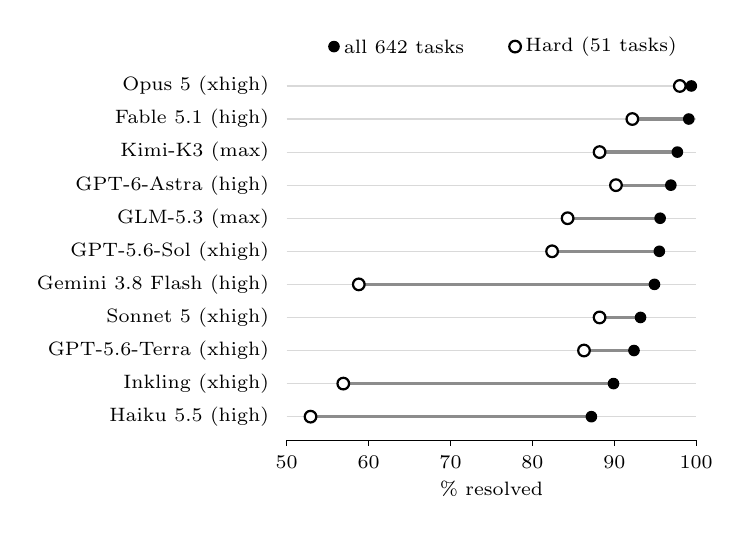
\begin{tikzpicture}
\node[anchor=east,font=\scriptsize] at (-0.1,0.00) {Opus 5 (xhigh)};
\draw[gray!30] (0,0.00) -- (5.2,0.00);
\draw[line width=1.2pt,black!45] (4.992,0.00) -- (5.138,0.00);
\fill[black] (5.138,0.00) circle (2.1pt);
\draw[black,fill=white,line width=0.8pt] (4.992,0.00) circle (2.1pt);
\node[anchor=east,font=\scriptsize] at (-0.1,-0.42) {Fable 5.1 (high)};
\draw[gray!30] (0,-0.42) -- (5.2,-0.42);
\draw[line width=1.2pt,black!45] (4.389,-0.42) -- (5.106,-0.42);
\fill[black] (5.106,-0.42) circle (2.1pt);
\draw[black,fill=white,line width=0.8pt] (4.389,-0.42) circle (2.1pt);
\node[anchor=east,font=\scriptsize] at (-0.1,-0.84) {Kimi-K3 (max)};
\draw[gray!30] (0,-0.84) -- (5.2,-0.84);
\draw[line width=1.2pt,black!45] (3.973,-0.84) -- (4.961,-0.84);
\fill[black] (4.961,-0.84) circle (2.1pt);
\draw[black,fill=white,line width=0.8pt] (3.973,-0.84) circle (2.1pt);
\node[anchor=east,font=\scriptsize] at (-0.1,-1.26) {GPT-6-Astra (high)};
\draw[gray!30] (0,-1.26) -- (5.2,-1.26);
\draw[line width=1.2pt,black!45] (4.181,-1.26) -- (4.878,-1.26);
\fill[black] (4.878,-1.26) circle (2.1pt);
\draw[black,fill=white,line width=0.8pt] (4.181,-1.26) circle (2.1pt);
\node[anchor=east,font=\scriptsize] at (-0.1,-1.68) {GLM-5.3 (max)};
\draw[gray!30] (0,-1.68) -- (5.2,-1.68);
\draw[line width=1.2pt,black!45] (3.567,-1.68) -- (4.742,-1.68);
\fill[black] (4.742,-1.68) circle (2.1pt);
\draw[black,fill=white,line width=0.8pt] (3.567,-1.68) circle (2.1pt);
\node[anchor=east,font=\scriptsize] at (-0.1,-2.10) {GPT-5.6-Sol (xhigh)};
\draw[gray!30] (0,-2.10) -- (5.2,-2.10);
\draw[line width=1.2pt,black!45] (3.370,-2.10) -- (4.732,-2.10);
\fill[black] (4.732,-2.10) circle (2.1pt);
\draw[black,fill=white,line width=0.8pt] (3.370,-2.10) circle (2.1pt);
\node[anchor=east,font=\scriptsize] at (-0.1,-2.52) {Gemini 3.8 Flash (high)};
\draw[gray!30] (0,-2.52) -- (5.2,-2.52);
\draw[line width=1.2pt,black!45] (0.915,-2.52) -- (4.670,-2.52);
\fill[black] (4.670,-2.52) circle (2.1pt);
\draw[black,fill=white,line width=0.8pt] (0.915,-2.52) circle (2.1pt);
\node[anchor=east,font=\scriptsize] at (-0.1,-2.94) {Sonnet 5 (xhigh)};
\draw[gray!30] (0,-2.94) -- (5.2,-2.94);
\draw[line width=1.2pt,black!45] (3.973,-2.94) -- (4.493,-2.94);
\fill[black] (4.493,-2.94) circle (2.1pt);
\draw[black,fill=white,line width=0.8pt] (3.973,-2.94) circle (2.1pt);
\node[anchor=east,font=\scriptsize] at (-0.1,-3.36) {GPT-5.6-Terra (xhigh)};
\draw[gray!30] (0,-3.36) -- (5.2,-3.36);
\draw[line width=1.2pt,black!45] (3.775,-3.36) -- (4.410,-3.36);
\fill[black] (4.410,-3.36) circle (2.1pt);
\draw[black,fill=white,line width=0.8pt] (3.775,-3.36) circle (2.1pt);
\node[anchor=east,font=\scriptsize] at (-0.1,-3.78) {Inkling (xhigh)};
\draw[gray!30] (0,-3.78) -- (5.2,-3.78);
\draw[line width=1.2pt,black!45] (0.718,-3.78) -- (4.150,-3.78);
\fill[black] (4.150,-3.78) circle (2.1pt);
\draw[black,fill=white,line width=0.8pt] (0.718,-3.78) circle (2.1pt);
\node[anchor=east,font=\scriptsize] at (-0.1,-4.20) {Haiku 5.5 (high)};
\draw[gray!30] (0,-4.20) -- (5.2,-4.20);
\draw[line width=1.2pt,black!45] (0.302,-4.20) -- (3.869,-4.20);
\fill[black] (3.869,-4.20) circle (2.1pt);
\draw[black,fill=white,line width=0.8pt] (0.302,-4.20) circle (2.1pt);
\draw (0,-4.50) -- (5.2,-4.50);
\draw (0.000,-4.50) -- (0.000,-4.57) node[below,font=\scriptsize] {50};
\draw (1.040,-4.50) -- (1.040,-4.57) node[below,font=\scriptsize] {60};
\draw (2.080,-4.50) -- (2.080,-4.57) node[below,font=\scriptsize] {70};
\draw (3.120,-4.50) -- (3.120,-4.57) node[below,font=\scriptsize] {80};
\draw (4.160,-4.50) -- (4.160,-4.57) node[below,font=\scriptsize] {90};
\draw (5.200,-4.50) -- (5.200,-4.57) node[below,font=\scriptsize] {100};
\node[font=\scriptsize] at (2.60,-5.12) {\% resolved};
\fill[black] (0.6,0.5) circle (2.1pt) node[right,font=\scriptsize] {all 642 tasks};
\draw[black,fill=white,line width=0.8pt] (2.9,0.5) circle (2.1pt) node[right,font=\scriptsize] {Hard (51 tasks)};
\end{tikzpicture}}
\caption{Percent of tasks resolved on SWE-Bench Pro V2 (filled dots) and its Hard split (open dots). The full set separates these systems by about 12 points (87.2--99.4\%) while the Hard split spans from 52.9\% to 98.0\%.}
\label{fig:spread}
\end{figure}

\section{Related Work}
\label{sec:related}

\paragraph{Benchmarks for computer-use agents.} Interactive benchmarks evaluate CUAs on desktop operating systems \citep{xie2024osworld,bonatti2025windowsagentarena,yang2025macosworld,davydova2025osuniverse}, websites \citep{zhou2024webarena,koh2024visualwebarena,he2024webvoyager,xue2025illusion}, enterprise software \citep{drouin2024workarena,boisvert2024workarenapp,xu2024theagentcompany} and mobile apps \citep{rawles2025androidworld}, alongside offline trajectory datasets \citep{deng2023mind2web} and grounding tests \citep{li2025screenspotpro}. They judge the final state with deterministic checkers or rubric-based LLM judges \citep{xue2025illusion,lu2025agentrewardbench}, and they differ mainly in domain and horizon, up to tasks that take a person more than an hour \citep{yuan2026osworld2}. Time enters only as a step cap, and the cap itself shifts scores \citep{xlang2025osworldverified,qin2025uitars,agashe2025agents2}; AndroidWorld derives its per-task cap from human step counts \citep{rawles2025androidworld}. Robustness benchmarks add pop-ups and other everyday disruptions \citep{zhang2025popups,yang2026guirobust}, and PersonaCUABench finds that many fully completed runs still fall short of the requesting persona's satisfaction \citep{li2026personacuabench}. \bench keeps deterministic end-state checks, but a correct end state is not enough: the run must also stay within a human-labelled tolerance.

\paragraph{Efficiency, speed and reliability.} A growing body of work argues that accuracy alone misrepresents agents. Accounting for cost \citep{kapoor2025agentsthatmatter,kapoor2026hal}, consistency across repeated runs \citep{yao2025taubench,rabanser2026reliability} and benchmark rigour \citep{zhu2025abc} each changes the conclusions drawn from pass rates. For CUAs, OSWorld-Human annotates a human trajectory for every OSWorld task and finds that the best agents take 2.7--4.3$\times$ more steps than necessary, with end-to-end latencies of tens of minutes \citep{abhyankar2026osworldhuman}. cua-speedrun standardizes the infrastructure for timing CUAs and finds that frontier agents spend 86--127\,s per OSWorld task \citep{aggarwal2026cuaspeedrun}. ComponentBench pairs 2,910 programmatically generated UI-component tasks with human reference trajectories, and even its fastest agent configuration takes 3.7$\times$ as long as the matched human \citep{guan2026componentbench}. METR measures agent capability by the human completion time of the tasks agents can do \citep{kwa2025metr}, and ARC-AGI-3 scores agents by their action efficiency relative to humans on abstract games \citep{arcprize2026arcagi3}. These works use human effort as a reference for efficiency or difficulty. We also ask annotators how much more than their own effort they would tolerate from an agent, and we use that tolerance as a pass/fail boundary on realistic, human-written tasks.

\paragraph{Easy for people, hard for agents.} Benchmarks made of tasks that people solve easily expose gaps that hard tasks hide, including web games \citep{thomas2025webgames}, web browsing questions \citep{song2025bearcubs}, abstract reasoning puzzles \citep{chollet2019measure,chollet2025arcagi2,arcprize2026arcagi3} and commonsense questions \citep{simplebench2024}. The pattern echoes Moravec's paradox \citep{moravec1988mind}: the perception and motor skills that people exercise without effort are among the hardest to automate. \bench applies this design to ordinary interactions in ordinary applications, and asks both whether agents succeed at them and whether they do so before a person would give up.

\paragraph{Failure modes of agents.} Taxonomies of agent failures \citep{cemri2025mast,zhu2025agentdebug} and studies of overthinking, in which reasoning models spend far more computation on easy problems than they need \citep{chen2025overthinking,cuadron2025danger}, explain why agents fail or waste effort. For GUI agents, repetitive loops and premature stopping recur as dominant failure modes \citep{koh2024visualwebarena,han2026vlaagui,wei2026steplevel}, and AgentRewardBench labels repetitiveness alongside success and side effects \citep{lu2025agentrewardbench}. These taxonomies are organized around the agent's internal errors. Our frustration patterns (\S\ref{sec:patterns}) are organized around what the user sees, and they include patterns such as stalling and detours that a correctness criterion does not penalize at all.

\paragraph{User frustration and tolerance.} HCI research defines frustration as the appraisal of an interface as an obstacle to a goal \citep{bessiere2006model}, and diary studies found that it costs users a third to a half of their time at the computer \citep{ceaparu2004frustration,lazar2006severity}. Waiting is a central cause. Classic response-time limits place the end of uninterrupted attention at about ten seconds \citep{miller1968response,card1991information,nielsen1993usability}, web users tolerate about two seconds when retrieving information \citep{nah2004tolerable}, and task performance and the intention to return drop with delays of a few seconds \citep{galletta2004delays}. Expectations come from how long a task usually takes, so a result that takes far longer than expected frustrates \citep{shneiderman1984response}, and direct-manipulation tasks require faster responses than conversational ones \citep{dabrowski2011forty}. Human effort can be predicted from operator times with the Keystroke-Level Model and GOMS \citep{card1980keystroke,card1983psychology}; we measure it directly instead. People stop relying on automation after they observe it err \citep{parasuraman1997humans,lee2004trust,dietvorst2015algorithm}, and guidelines for human-AI interaction call for efficient dismissal and correction of an assistant \citep{horvitz1999principles,amershi2019guidelines}. Recent studies of LLM agents find that latency is a main complaint and a reason users take over \citep{mozannar2025magentic,maslych2025mitigating}, that deployed agents loop and run slower than doing the task by hand \citep{shome2026johnny,zhang2025unintended}, and that oversight depends on when control passes between user and agent \citep{huq2025cowpilot,huq2026modeling,chen2026oversight}. Tolerance for delay also depends on the task \citep{tan2026latency}. We therefore label tolerance per task instead of assuming a global limit, and we use it as the boundary between an acceptable and a frustrating run.

% Preamble: \usepackage{booktabs,tabularx,graphicx,tikz}
%           \usetikzlibrary{positioning,arrows.meta,calc}
\section{Methodology}
\label{sec:method}

We start from the 731 tasks of SWE-Bench Pro Public v1.0. A task consists of an instruction (problem statement, requirements, new interfaces), a container image with the repository at its base commit, a reference patch, a hidden test patch, fail-to-pass and pass-to-pass lists naming the graded tests, and a verifier that applies the test patch, runs the tests and parses the output. A task is valid if every solution that satisfies the instruction passes and every solution that does not, fails. Figure~\ref{fig:pipeline} traces the tasks through three repair rounds, an engineer review and a final review. Round~1 repaired 40 container images whose reference patches carried test and fixture files or whose instructions lacked the standard template. Round~2 ran an automated audit of difficulty calibration, instruction--test alignment and reward hacking; it flagged 387 tasks (53\%), found 326 clean and errored on 18. Engineers revised the flagged tasks to align instructions with the graded tests and to cover the stated requirements, re-auditing each batch, until about 700 passed; about 30 could not be made to pass through task edits alone. Three changes applied to every task: the \textit{``do not edit tests''} constraint left the instruction template and the verifier now reverts test-related changes before applying the test patch; git history was scrubbed from the images so that agents cannot recover the fix; and network access was disabled in the agent phase, after a frontier model copied reference solutions verbatim from GitHub on 351 solved tasks, only 237 of which held up with GitHub blocked. The result kept all 731 tasks. Round~3 ran two agentic audits (\S\ref{sec:audits}), which flagged 200 tasks (27\%). Engineers adjudicated every flag (\S\ref{sec:review}): 68 tasks were repaired, 43 kept unchanged and 89 discarded. A final review extended task-specific edits across the whole set, and the shared verifier was hardened for every task (\S\ref{sec:verifier}). The release has 642 tasks, 391 of which carry a task-specific repair (Table~\ref{tab:repairs-discards}): 480 of the 731 tasks (66\%) were repaired or removed, the other 251 changed only through the verifier hardening, and no reference solution was changed.

% Pipeline figure for Section~\ref{sec:method}: flow of the 731 tasks from
% SWE-Bench Pro v1.0 to the 642 released tasks.
% Band and bar heights are proportional to task counts (0.046 mm per task).
% Preamble: \usepackage{tikz,graphicx} (xcolor is loaded by tikz)
\definecolor{sbpFlag}{HTML}{4C72B0}
\definecolor{sbpRep}{HTML}{55A868}
\definecolor{sbpDisc}{HTML}{C44E52}
\definecolor{sbpKeep}{HTML}{7F7F7F}
\definecolor{sbpNone}{HTML}{B0B0B0}
\definecolor{sbpImg}{HTML}{8172B3}
\definecolor{sbpErr}{HTML}{DD8452}
\definecolor{sbpRes}{HTML}{64B5CD}
\begin{figure*}[t]
\centering
\resizebox{\textwidth}{!}{%
\begin{tikzpicture}[x=1mm, y=1mm, font=\sffamily\scriptsize,
  execute at begin node={\hyphenpenalty=10000\exhyphenpenalty=10000}]
% ---------------------------------------------------------------- bands
% Input -> Round 1: untouched / image repairs
\fill[sbpNone!22] (2.2,-1.92) .. controls (12.1,-1.92) and (12.1,0) .. (22,0)
  -- (22,-31.786) .. controls (12.1,-31.786) and (12.1,-33.706) .. (2.2,-33.706) -- cycle;
\fill[sbpImg!22] (2.2,-33.706) .. controls (12.1,-33.706) and (12.1,-31.786) .. (22,-31.786)
  -- (22,-33.626) .. controls (12.1,-33.626) and (12.1,-35.546) .. (2.2,-35.546) -- cycle;
% Round 1 -> Round 2
\fill[sbpNone!22] (24.2,0) .. controls (34.1,0) and (34.1,-1.53) .. (44,-1.53)
  -- (44,-33.316) .. controls (34.1,-33.316) and (34.1,-31.786) .. (24.2,-31.786) -- cycle;
\fill[sbpImg!22] (24.2,-31.786) .. controls (34.1,-31.786) and (34.1,-33.316) .. (44,-33.316)
  -- (44,-35.156) .. controls (34.1,-35.156) and (34.1,-33.626) .. (24.2,-33.626) -- cycle;
% Round 2 -> Result: flagged / clean / audit errors
\fill[sbpFlag!22] (46.2,-1.53) .. controls (57.1,-1.53) and (57.1,-0.51) .. (68,-0.51)
  -- (68,-18.312) .. controls (57.1,-18.312) and (57.1,-19.332) .. (46.2,-19.332) -- cycle;
\fill[sbpNone!22] (46.2,-19.332) .. controls (57.1,-19.332) and (57.1,-18.312) .. (68,-18.312)
  -- (68,-33.308) .. controls (57.1,-33.308) and (57.1,-34.328) .. (46.2,-34.328) -- cycle;
\fill[sbpErr!30] (46.2,-34.328) .. controls (57.1,-34.328) and (57.1,-33.308) .. (68,-33.308)
  -- (68,-34.136) .. controls (57.1,-34.136) and (57.1,-35.156) .. (46.2,-35.156) -- cycle;
% Result -> Round 3: unflagged / flagged
\fill[sbpNone!22] (70.2,-0.51) .. controls (81.1,-0.51) and (81.1,-2.04) .. (92,-2.04)
  -- (92,-26.466) .. controls (81.1,-26.466) and (81.1,-24.936) .. (70.2,-24.936) -- cycle;
\fill[sbpFlag!22] (70.2,-24.936) .. controls (81.1,-24.936) and (81.1,-26.466) .. (92,-26.466)
  -- (92,-35.666) .. controls (81.1,-35.666) and (81.1,-34.136) .. (70.2,-34.136) -- cycle;
% Round 3 -> Release: never flagged, bypasses engineer review
\fill[sbpNone!22] (94.2,-2.04) .. controls (121.1,-2.04) and (121.1,-3.58) .. (148,-3.58)
  -- (148,-28.006) .. controls (121.1,-28.006) and (121.1,-26.466) .. (94.2,-26.466) -- cycle;
% Round 3 -> Engineer review: repaired / kept / discarded
\fill[sbpRep!22] (94.2,-26.466) .. controls (107.1,-26.466) and (107.1,-28.7) .. (120,-28.7)
  -- (120,-31.736) .. controls (107.1,-31.736) and (107.1,-29.502) .. (94.2,-29.502) -- cycle;
\fill[sbpKeep!22] (94.2,-29.502) .. controls (107.1,-29.502) and (107.1,-31.736) .. (120,-31.736)
  -- (120,-33.806) .. controls (107.1,-33.806) and (107.1,-31.572) .. (94.2,-31.572) -- cycle;
\fill[sbpDisc!22] (94.2,-31.572) .. controls (107.1,-31.572) and (107.1,-33.806) .. (120,-33.806)
  -- (120,-37.9) .. controls (107.1,-37.9) and (107.1,-35.666) .. (94.2,-35.666) -- cycle;
% Engineer review -> Release
\fill[sbpRep!22] (122.2,-28.7) .. controls (135.1,-28.7) and (135.1,-28.006) .. (148,-28.006)
  -- (148,-31.042) .. controls (135.1,-31.042) and (135.1,-31.736) .. (122.2,-31.736) -- cycle;
\fill[sbpKeep!22] (122.2,-31.736) .. controls (135.1,-31.736) and (135.1,-31.042) .. (148,-31.042)
  -- (148,-33.112) .. controls (135.1,-33.112) and (135.1,-33.806) .. (122.2,-33.806) -- cycle;
% ---------------------------------------------------------------- nodes
\fill[black!70] (0,-35.546) rectangle (2.2,-1.92);
\fill[sbpNone]  (22,-31.786) rectangle (24.2,0);
\fill[sbpImg]   (22,-33.626) rectangle (24.2,-31.786);
\fill[sbpFlag]  (44,-19.332) rectangle (46.2,-1.53);
\fill[sbpNone]  (44,-34.328) rectangle (46.2,-19.332);
\fill[sbpErr]   (44,-35.156) rectangle (46.2,-34.328);
\fill[sbpRes]   (68,-34.136) rectangle (70.2,-0.51);
\fill[sbpNone]  (92,-26.466) rectangle (94.2,-2.04);
\fill[sbpFlag]  (92,-35.666) rectangle (94.2,-26.466);
\fill[sbpRep]   (120,-31.736) rectangle (122.2,-28.7);
\fill[sbpKeep]  (120,-33.806) rectangle (122.2,-31.736);
\fill[sbpDisc]  (120,-37.9) rectangle (122.2,-33.806);
\fill[sbpNone]  (148,-28.006) rectangle (150.2,-3.58);
\fill[sbpRep]   (148,-31.042) rectangle (150.2,-28.006);
\fill[sbpKeep]  (148,-33.112) rectangle (150.2,-31.042);
% ---------------------------------------------------------------- labels
\node[anchor=north west, inner sep=1pt] at (0,-36.3) {\textbf{731} tasks};
\node[align=center] at (12.1,-17.8) {\textbf{691}\\untouched};
\node[anchor=north west, inner sep=1pt] at (22,-35.0) {\textbf{40} repaired};
\node[align=center] at (57.1,-9.9) {\textbf{387}\\flagged and fixed};
\node[align=center] at (57.1,-26.3) {\textbf{326}\\clean};
\node[anchor=north west, inner sep=1pt] at (44,-35.8) {\textbf{18} errors};
\node[align=center] at (81.1,-13.5) {\textbf{531}\\unflagged};
\node[align=center] at (81.1,-30.3) {\textbf{200}\\flagged};
\node[anchor=west, inner sep=1pt] at (123.4,-29.9) {\textbf{68} repaired};
\node[anchor=west, inner sep=1pt] at (123.4,-33.0) {\textbf{43} kept};
\node[anchor=west, inner sep=1pt] at (123.4,-35.9) {\textbf{89} discarded};
\node[anchor=west, inner sep=1pt] at (151.4,-6.5) {\textbf{642} released};
% ---------------------------------------------------------------- stage headers
\node[anchor=north west, inner sep=0pt, text width=20mm, align=left] at (0,21)
  {{\bfseries Input}\\[1.5pt]\textcolor{black!65}{SWE-Bench Pro\\v1.0}};
\node[anchor=north west, inner sep=0pt, text width=20mm, align=left] at (22,21)
  {{\bfseries Round 1}\\[1.5pt]\textcolor{black!65}{Image repairs}};
\node[anchor=north west, inner sep=0pt, text width=22mm, align=left] at (44,21)
  {{\bfseries Round 2}\\[1.5pt]\textcolor{black!65}{Automated audits}};
\node[anchor=north west, inner sep=0pt, text width=22mm, align=left] at (68,21)
  {{\bfseries Round 3}\\[1.5pt]\textcolor{black!65}{Agentic audits\\artifact audit (161 flagged)\\failure audit (54 flagged; 39 new)}};
\node[anchor=north west, inner sep=0pt, text width=26mm, align=left] at (92,21)
  {{\bfseries Engineer review}\\[1.5pt]\textcolor{black!65}{verdict on every flag\\blind check of\\every repair}};
\node[anchor=north west, inner sep=0pt, text width=26mm, align=left] at (120,21)
  {{\bfseries Final review}\\[1.5pt]\textcolor{black!65}{every flag was\\cross-checked}};
\node[anchor=north west, inner sep=0pt, text width=24mm, align=left] at (148,21)
  {{\bfseries Release}\\[1.5pt]\textcolor{black!65}{verifier hardened\\for all tasks}};
\end{tikzpicture}}%
\caption{Flow of the 731 tasks from SWE-Bench Pro v1.0 to the released set;
bar and band heights are proportional to task counts. Round~1 repairs 40
container images (leaked test and fixture files, non-standard instructions).
Round~2's automated audit flags 387 tasks (all fixed by human experts). In Round~3, the artifact audit (an LLM agent and a human
auditor compare the instruction with the tests and reference patch) and the
failure audit (an LLM judge attributes failed runs of four agent setups) flag
200 tasks. Engineers adjudicate every flag, and a repair ships only after a
blind re-implementation of the edited instruction passes the hidden tests.}
\label{fig:pipeline}
\end{figure*}

\subsection{Agentic audits}
\label{sec:audits}

\paragraph{Artifact audit.}
An LLM agent compared each task's instruction with its test lists and reference patch, without executing anything. It flagged six patterns: test requirements missing from the instruction, instruction statements contradicted by the tests, test or solution detail copied into the instruction, changed behaviour that no graded test exercises, fixtures read by the tests but never created, and graded lists naming a whole test file. Overly verbose requirement sections were a leakage signal, as they often transcribed the reference patch. A human auditor reviewed the flags and marked high-priority cases; 161 tasks were flagged.

\paragraph{Failure audit.}
We ran four agent configurations on every task: Claude Code with Claude Opus~5, Codex with GPT-5.6, and mini-SWE-agent with both models. For each run, an LLM judge read the trajectory, patch, verifier log and graded tests and attributed each failure to the model or to the task. A task was flagged when a patch consistent with a reasonable reading of the instruction was rejected. For example, in a \textit{vuls} task two configurations fell back to the bundle directory name as instructed and reported \texttt{Sample.app}, while the graded test expects \texttt{Sample} because the reference patch strips the suffix without the instruction saying so. For each such flag we record the defect type, the fix location, an effort estimate, a proposed edit, and the passing and failing configurations. The failure audit flagged 54 tasks, 39 of them new, for 200 flagged tasks in all.


\subsection{Defect taxonomy}
\label{sec:taxonomy}

We merged the audits' labels and the final review's edit types into the six categories of Table~\ref{tab:repairs-discards}; each task is counted once, under its main edit (instruction, else test patch, else grading files). Unstated requirements, contradictions and verifier or environment defects make correct solutions fail; leakage and insufficient tests make a task easier than intended or let an incomplete solution pass.

\begin{table}[t]
\centering
\small
\setlength{\tabcolsep}{3pt}
\begin{tabularx}{\columnwidth}{@{}>{\raggedright\arraybackslash}p{2.05cm} >{\raggedright\arraybackslash}X r r@{}}
\toprule
\textbf{Category} & \textbf{Description} & \textbf{Rep.} & \textbf{Disc.} \\
\midrule
Solution leakage & The instruction gives away test or solution detail. & 18 & 4 \\
\addlinespace
Spec--test contradiction & The instruction contradicts what the tests check. & 10 & 5 \\
\addlinespace
Unstated test requirement & The tests require behaviour, names or files the instruction never states. & 119 & 22 \\
\addlinespace
Insufficient tests & The tests miss part of the change or check incidental details instead of behaviour. & 1 & 33 \\
\addlinespace
Verifier or environment defect & The grading setup or container decides the score regardless of the solution. & 228 & 19 \\
\addlinespace
Miscellaneous & -- & 15 & 6 \\
\midrule
\textbf{Total} & & \textbf{391} & \textbf{89} \\
\bottomrule
\end{tabularx}
\caption{Defect categories of tasks repaired and kept (Rep.) and discarded (Disc.) between the 731 tasks of SWE-Bench Pro Public v1.0 and the final 642. Together, 480 of the 731 tasks (66\%) were repaired or removed. Each task is counted once, under the defect its main edit addresses. Every task also received the hardened verifier, and no reference solution was changed.}
\label{tab:repairs-discards}
\end{table}

\paragraph{Unstated test requirement (119 repaired, 22 discarded).}
The tests depend on behaviour, names or files the instruction does not mention; the \textit{vuls} task above was repaired by stating that the \texttt{.app} suffix is removed. Most of the 119 repairs (25 from confirmed flags, 94 from the final review) are short additions stating something the graded tests already enforce: an exact value, string, ordering or signature. A task was discarded when the test checks how the reference patch happens to be written, stating that would give the solution away.

\paragraph{Spec--test contradiction (10 repaired, 5 discarded).}
The instruction says one thing and the graded test checks another. Wrong instructions were corrected (8 from flags, 2 in the final review); contradictions whose fix lies in the tests were discarded, for example a \textit{webclients} task whose interface declares an \texttt{Element} argument while the graded test passes a \texttt{Document}.

\paragraph{Solution leakage (18 repaired, 4 discarded).}
Leaky instructions walked through the reference patch file by file, or copied expected values from the tests. A \textit{tutanota} instruction told the agent to update the try-catch block around \texttt{aes256Decrypt} in \texttt{decrypt}; the repaired version specifies behaviour only: a \texttt{CryptoError} raised by the crypto library must surface as the application's own \texttt{CryptoError}, which the credentials layer converts to \texttt{KeyPermanentlyInvalidatedError}. Repairs delete the leaked text and, where a test depends on it, restate the requirement as behaviour. The four discards were repaired and then removed before release (\S\ref{sec:review}).

\paragraph{Insufficient tests (1 repaired, 33 discarded).}
The graded tests leave part of the change unchecked: in a \textit{flipt} task they cover only the error paths of a new cache layer, so a \texttt{getJSON} that always returns false and a no-op \texttt{setJSON} pass. Engineers did not write new tests, so these tasks were discarded; the one repair adds a single assertion to a \textit{teleport} test.

\paragraph{Verifier or environment defect (228 repaired, 19 discarded).}
In 16 discarded tasks the fail-to-pass list names a whole file (e.g.\ \texttt{test/tests/calendar/\allowbreak CalendarUtilsTest.js \textbar{} test suite}), so any unrelated or flaky failure in that file fails a correct patch; in 3 the image prevents grading, for example a \textit{teleport} test skipped because SoftHSM is missing, which the verifier scores as a failure. The 228 repaired tasks are those whose only task-specific change was to grading files (223): run scripts narrowed from the whole repository to the package with the graded tests in the four Go repositories, parsers, and the graded-test names of 20 \textit{element-web} tasks; plus 5 instructions that gained an environment fact such as the absence of network or an exact dependency version. Shared verifier defects were fixed for all tasks (\S\ref{sec:verifier}).

\paragraph{Miscellaneous (15 repaired, 6 discarded).}
Fifteen instructions were reworded or given implementation detail that fixes no defect. The six discarded tasks had no flag that held: two \textit{ansible} tasks were quarantined after a leakage flag was rejected, and four were repaired and dropped although their recorded flag did not hold.


\subsection{Engineer review}
\label{sec:review}

Engineers applied one criteria: if the reference patch adds a behaviour that a hidden test checks, the instruction must state the behaviour, but not how the reference patch implements it. Tests were not edited to agree with an instruction, and instructions were never rewritten to match wrong tests.

23 contracted engineers adjudicated every flag in 404 hours. For each claim they recorded whether it holds, holds in part or does not hold, citing artifact and line (e.g.\ \texttt{test\_patch\_before:178}); high-priority flags received a second independent review and a third pass by the project team. A flag that did not hold left the task unchanged (45 tasks; 26 of these rejected flags claimed solution leakage, the type that most often did not hold). A flag whose gap was in the instruction led to an edit limited to where the flag held (69 tasks, 53 of them in the release). A flag whose remedy lay in the tests, fixtures, verifier or image led to quarantine (73 tasks, mostly insufficient tests, 32, and verifier or environment defects, 19). Engineers corrected 55 tasks in all: 51 for a flag that held in full or in part (18 solution leakage, 8 spec--test contradiction, 25 unstated requirement) and 4 for a flag that a later review rejected, which remain in the release through their other edits. With the final review's edits to flagged tasks, 68 of the 200 flagged tasks carry an edit, 43 are unchanged and 89 were discarded (Figure~\ref{fig:pipeline}).

Repairs were validated blind: a second engineer who had seen neither the original task nor the reference patch implemented the edited instruction, and the edit shipped only if that implementation passed the hidden tests. Sixteen repaired tasks were removed before release; we count them as discards under their original flag, and they include all four leakage discards.

\paragraph{Final review.}
Before release, a final pass cross-checked every flag and reviewed the whole set, making task-specific edits to 340 further tasks: 116 instruction edits, one test patch with an added assertion and grading-file changes on 223 tasks, distributed over the rows of Table~\ref{tab:repairs-discards} as given above. A task counts as repaired in the table if one of its own files changed between v1.0 and the release (instruction, test patch, graded-test list, parser or run script); changes applied identically to every task (\texttt{test.sh}, the Dockerfile, \texttt{task.toml} and the pytest worker pin) are not counted.


\subsection{Verifier hardening}
\label{sec:verifier}

Defects in shared grading code were fixed for all tasks; per-task grading files that changed form the verifier row of Table~\ref{tab:repairs-discards} where they were a task's only change.

\paragraph{Scoping and resources.}
The Go verifier ran \texttt{go test ./...} over the whole repository. Scoping it to the graded packages on 253 tasks removed out-of-memory failures and timeouts. Run scripts on 231 tasks that executed the full suite were restricted to the graded tests. With automatic worker counts, pytest-xdist spawned up to 128 workers on small test files and crashed with ``no tests ran'': we capped it at four workers on 239 tasks and inside \texttt{ansible-test} on 83.

\paragraph{Parsing and environment.}
The jest parser assigned tests in failing files to the wrong file and dropped failures (47 tasks), and it truncated test titles at the first parenthesis: it now strips only the trailing timing. We added kernel headers for cgo builds (5 tasks), fetched at grading time one Go module missing from an image's offline cache, re-derived test scoping on 3 tasks that omitted the packages defining the graded tests, and restored CRLF line endings in a fixture that made the reference patch fail.

\paragraph{Test-file reset.}
Before the hidden tests run, the verifier (i)~restores every path the test patch touches and deletes only paths it creates; (ii)~restores modified tracked test data (test data, fixtures, mocks, snapshots), with allowlists for the six reference patches that change fixtures; (iii)~removes agent-written test files that collide with hidden tests; (iv)~clears stale git lock files left by killed agent commands; and (v)~deletes \texttt{\_\_pycache\_\_} and \texttt{.pyc} files. Without (i), agent edits to snapshots owned by the test patch made it fail to apply in 44 runs. Step (v) addresses \texttt{.pyc} files that an agent's \texttt{git stash} round trip left with unchanged size and timestamp, which made the verifier import the base code.

On the assembled 642-task set, the reference patch passes every task and the empty patch fails every task.


\subsection{Hardened evaluation protocol}
\label{sec:protocol}

We run every model under a \textit{locked protocol} where the harness sets network access per phase of a run, and grades the agent's patch in a fresh container rather than in the agent's sandbox.

\paragraph{Network.}
With the network open, 32 of 642 Claude Opus~5 trajectories contacted code hosts, and 25 downloaded the task's own repository. Under the lock, the sandbox can reach only the model endpoint during the agent phase (the allowlist names that hostname alone), web tools that scaffolds execute outside the sandbox are disabled, and the images carry no fixing commit in their git history.

\paragraph{Grading.}
The original harness ran the verifier in the sandbox the agent had just used. Because the verifier restores test files but not binaries, a scripted agent that edits no source file and replaces \texttt{python3} with a script printing \textsc{PASSED} scores 1. Forged dependencies pass through the same gap: with the network closed, some agents that could not fetch a fix edited the Go module cache in place or served a fabricated module version from a local \texttt{GOPROXY}, and neither change appears in the diff. We now save the agent's changes as a patch, apply it to a fresh copy of the task image, run the unchanged verifier there and report that grade, so that binaries or module caches do not carry over.
%We report both grades for every task. When the two disagree, two more fresh grades decide, by majority.
% CHECK: CHEATING_MODES.md says the fresh re-grade is authoritative and that flips are adjudicated with 2 extra fresh re-grades (a forgery fails 2/2, a flake passes at least 1/2). Align the commented sentence with that before re-enabling it.

\paragraph{Trajectory audits.}
A fresh re-grade cannot catch a forgery committed inside the patch, so we audit patches for \texttt{replace} directives that point into the patch or to absolute paths, \texttt{go.sum} entries for modules absent from the image, and large new directories that imitate a third-party SDK. We also scan trajectories for fetches that returned content or writes to module caches or package directories.
% CHECK: state whether flagged patches are rejected automatically or reviewed by hand.
\section{Experiments}
\label{sec:experiments}

\newcommand{\gfail}{\textcolor{red!70!black}{\ding{55}}}
\newcommand{\gpass}{\textcolor{green!40!black}{\ding{51}}}
\newcommand{\exlabel}[1]{\textsc{\scriptsize #1}}
\tcbset{exbox/.style={colback=black!3,colframe=black!35,boxrule=0.4pt,arc=1.5pt,
  left=4pt,right=4pt,top=3pt,bottom=3pt,fonttitle=\small\bfseries,coltitle=black,
  colbacktitle=black!10,titlerule=0pt,toptitle=1.5pt,bottomtitle=1.5pt}}


\begin{figure*}[t]
\footnotesize
\begin{minipage}[t]{0.49\textwidth}
\begin{tcolorbox}[exbox,title={A.\ Verifier repair\hfill\normalfont\texttt{flipt-af7a0be}}]
\textbf{Task.} Deprecate \texttt{tracing.jaeger.enabled} for a unified tracing config. Every correct patch also updates the all-options fixture \texttt{internal/config/testdata/advanced.yml}; Opus~5's edit:
\begin{center}\texttt{jaeger: enabled: true} $\;\rightarrow\;$ \texttt{enabled: true, backend: jaeger}\end{center}
The hidden test patch edits the same fixture at line~28.

\medskip
\begin{tabular}{@{}p{1.3cm}p{5.4cm}@{\hspace{3pt}}c@{}}
\exlabel{Old verifier} & Resets test code only; test data ``intentionally left alone''. \texttt{advanced.yml: patch does not apply} $\to$ \texttt{Failed to apply test patch}. Opus~5 and GLM-5.3 graded~0. & \gfail \\[3pt]
\exlabel{Hardened verifier} & Restores every path the test patch touches before applying it. \texttt{Applied patch advanced.yml cleanly}; \texttt{Passed tests: 8}. Same edit, both graded~1. & \gpass \\
\end{tabular}

\medskip
\textit{Extent.} 44 v1 runs failed this way, but none under the fixed verifier.
\end{tcolorbox}
\end{minipage}\hfill
\begin{minipage}[t]{0.49\textwidth}
\begin{tcolorbox}[exbox,title={B.\ Instruction repair\hfill\normalfont\texttt{vuls-1832b4ee}}]
\textbf{Task.} Scan installed macOS applications. The hidden test feeds an app at \texttt{/System/Applications/Sample.app} whose \texttt{CFBundleDisplayName} and \texttt{CFBundleName} cannot be read and expects
\begin{center}\texttt{"Sample": \{Name: "Sample", Version: "", Repository: ""\}}\end{center}
The reference strips \texttt{.app/Contents/Info.plist} and keeps the basename.

\medskip
\begin{tabular}{@{}p{1.3cm}p{5.4cm}@{\hspace{3pt}}c@{}}
\exlabel{v1 instruction} & ``preserve bundle identifiers and names exactly as returned, trimming only whitespace''. Agents keep \texttt{Sample.app} or the error text. No pre-repair run passes. & \gfail \\[3pt]
\exlabel{V2 instruction} & ``fall back \ldots\ to the name of the enclosing \texttt{.app} directory with its \texttt{.app} extension removed''; unreadable fields ``must be empty rather than carrying the unread-value text''. 5 of 5 systems pass. & \gpass \\
\end{tabular}

\medskip
\textit{Extent.} Of 27 instruction repairs, 18 were failed by every v1 configuration. 15 are now solved by all frontier systems.
\end{tcolorbox}
\end{minipage}
\caption{Why scores rise after repair, on two public tasks. Left: the old verifier applied the hidden test patch over the agent's working tree, so a correct patch that also edited a test fixture could not be graded. Right: the hidden test encoded a fallback the instruction never stated. No hidden test was changed in either case.}
\label{fig:why-scores-rise}
\end{figure*}


\subsection{Setup}
We run several models and agents on SWE Bench Pro V2 (Table~\ref{tab:main}). Claude and GPT models run in their developers' native scaffolds, Claude Code and Codex (with web tools disabled in the \textit{locked protocol}) while Gemini and open source models run with mini-swe-agent \citep{minisweagent2025} and other open harnesses. Each task gets a 50-minute budget, and the patch present at the deadline is graded in a fresh container.  Because results depend on the scaffold and effort setting as well as the model, we report them per system, defined as the combination of the three. We report 95\% Wilson intervals for all the runs. %Versions, flags and costs are in Appendix~\ref{app:repro}.

\begin{table}[t]
\centering\small\setlength{\tabcolsep}{4pt}
\resizebox{\columnwidth}{!}{%
\begin{tabular}{llrcr}
\toprule
System & Scaffold & V2 (642) & 95\% CI & Hard (51) \\
\midrule
%Opus 5.5 (xhigh) & Claude Code & 99.4 & [98.4, 99.8] & 96.1 \\
Opus 5 (xhigh) & Claude Code & 99.4 & [98.4, 99.8] & 98.0 \\
Fable 5.1 (high) & Claude Code & 99.1 & [98.6, 99.6] & 92.2 \\
Kimi-K3 (max) & mini-swe-agent & 97.5 & [96.0, 98.5] & 88.2 \\
GPT-6-Astra (high) & Codex & 96.9 & [95.8, 98.0] & 90.2 \\
% GPT-6.1-Sol (xhigh) & mini-swe-agent & 96.1 & [94.9, 97.4] & -- \\
GLM-5.3 (max) & mini-swe-agent & 95.6 & [93.8, 97.0] & 84.3 \\
GPT-5.6-Sol (xhigh) & Codex & 95.5 & [94.1, 96.9] & 82.4 \\
Gemini 3.8 Flash (high) & mini-swe-agent & 94.9 & [93.4, 96.3] & 58.8 \\
Sonnet 5 (xhigh) & Claude Code & 93.2 & [91.4, 94.9] & 88.2 \\
GPT-5.6-Terra (xhigh) & Codex & 92.4 & [90.6, 94.2] & 86.3 \\
Inkling (xhigh) & mini-swe-agent & 89.9 & [87.8, 92.0] & 56.9 \\
Haiku 5.5 (high) & mini-swe-agent & 87.2 & [84.9, 89.6] & 52.9 \\

\bottomrule
\end{tabular}}
\caption{Percent of tasks resolved by each model (reasoning effort) and agent, with 95\% confidence intervals on V2, and on the Hard Split (51 instances) respectively.}
\label{tab:main}
\end{table}

\subsection{Main Results}
\label{sec:main-results}
In Table~\ref{tab:main} we see the frontier models solve \textasciitilde 99\% of tasks, and each of the 642 tasks is solved by at least one of them, which independently confirms that every task is solvable. The best system Opus~5 (xhigh) with Claude Code fails four tasks. We also see that the Hard split of 51 tasks separates the frontier models from the rest clearly (\S\ref{sec:hard}). The time budget is binding for some systems: 78 of Gemini's runs reached the 50-minute limit, although 65 of those still passed with the patch present at the deadline.

%\paragraph{Robustness to instruction edits.} On the 413 tasks whose instructions were not edited in this way, Opus~5 resolves 99.0\%, its full-set rate. Most of the remaining failures are attributable to the model. We audited all 33 tasks that Gemini failed. The reference patch passes all of them, two extra fresh grades of each failing patch changed no grade (0/66), and Opus~5 solves 29 of the 33. The audit attributes 23 failures to the model, 7 to borderline readings of the instruction and only 3 to residual task defects; excluding those three tasks changes Gemini's score from 94.9\% to 95.3\%.

\subsection{The Hard split}
\label{sec:hard}
We select the hard split based on model failures and another round of expert audits and settle on 51 tasks (Appendix \ref{app:hard}). On Hard, the model runs range from 52.9\% to 98.0\% (Table~\ref{tab:main}). Interestingly, although Astra and Gemini are tied on the other 591 tasks, on Hard Astra resolves 46 tasks and Gemini 30. Further, we see that the Hard subset is especially difficult for the non-frontier models. Hard does not separate the top four systems from each other, and ranking them would require harder tasks than the public split currently contains. 


\paragraph{Why the scores rise.} Figure~\ref{fig:why-scores-rise} shows one task per mechanism. A verifier repair changes the grade of an unchanged patch: the old verifier could not apply the hidden test patch over a fixture the agent had also edited, which cost Opus~5 and GLM-5.3 44 runs on v1 and none under the hardened verifier. An instruction repair changes what the agent builds: once the \texttt{.app} fallback was stated, all five systems solved a task no v1 configuration had solved before.


% \subsection{Do the data repairs matter?}
% \label{sec:private}
% \begin{table}[t]
\centering\small\setlength{\tabcolsep}{3pt}
\resizebox{\columnwidth}{!}{%
\begin{tabular}{lccc}
\toprule
System & As shipped & Verifier fixed & Fully fixed \\
\midrule
Opus 5 (xhigh) & 81.6 & 88.2 & \textbf{93.0} \\
Kimi K3 (max) & 78.7 & 84.2 & \textbf{88.2} \\
GLM-5.3 (max) & 77.6 & 83.1 & \textbf{87.9} \\
Gemini 3.8 Flash & 77.6 & 83.5 & \textbf{86.0} \\
Inkling (xhigh) & 67.6 & 71.3 & \textbf{79.0} \\
\bottomrule
\end{tabular}}
\caption{The never-public set (272 tasks), percent resolved. The middle column re-grades the same patches with the fixed verifier. The last column re-runs all systems after 68 instructions were corrected and the images rebuilt.}
\label{tab:private}
\end{table}

% Public-split scores alone cannot show that the repairs matter, because the failure audit chose some repairs after seeing failures. We therefore applied the same fixes to a never-public set of 272 tasks from the private repositories of 4 organisations (Table~\ref{tab:private}, Appendix~\ref{app:private}). Here the instruction audit was model-blind. An LLM judge saw each instruction, its hidden tests and the reference patch but no model output, and engineers corrected the 68 instructions it flagged as unclear about what the tests check.

% The score changes are concentrated on the repaired tasks. Fixing the shared verifier alone raised Opus~5 from 81.6\% to 88.2\%, and correcting the instructions and rebuilding the images raised it to 93.0\%. On the 68 corrected tasks, the pass rate pooled over five systems rose from 56.8\% to 73.2\%, while on the other 204 tasks it moved from 90.5\% to 91.4\%. On the repaired set, Opus~5 beats every other system (Holm $p\leq0.043$), and the five systems span 79.0--93.0\%. One exploit evaded re-grading on this set. On two tasks that need an SDK missing from the images, three systems wrote an imitation SDK into the patch, which passed because the tests mock the client; counting those 5 passes as failures lowers no score by more than 0.8 points. \jeff{should we have as section discussing why the scores increased? e.g. it would be great to pick out one task as an example, where a model that previously failed on the task passes  now due to fixed verifier and instructions}

\begin{table}[t]
\centering\small\setlength{\tabcolsep}{4pt}
\resizebox{\columnwidth}{!}{%
\begin{tabular}{lcccc}
\toprule
Model (effort) & mini-swe-agent & Pi & OpenCode & Spread \\
\midrule
GLM-5.3 (thinking) & 95.6 / 43 & 96.6 / 44 & 96.4 / 44 & 0.9 \\
Kimi K3 (max)      & 97.5 / 45 & 96.0 / 41 & 97.7 / 45 & 1.7 \\
Inkling (xhigh)    & 89.9 / 29 & 84.1 / 21 & 91.6 / 32 & 7.5 \\
\bottomrule
\end{tabular}}
\caption{The same model under three scaffolds. Each cell gives the percent of the 642 V2 tasks resolved and the number of Hard tasks resolved (of 51). Spread is the difference in V2 points between the model's best and worst scaffold.}
\label{tab:harness}
\end{table}


\begin{figure*}[t]
\centering
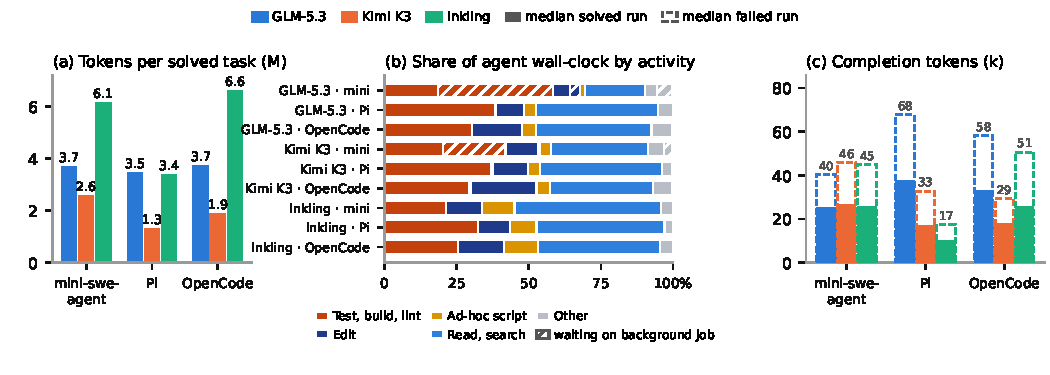
\includegraphics[width=\textwidth]{figures/harness_body.pdf}
\caption{The same model under three scaffolds. (a) Total tokens per solved task. (b) Share of agent wall-clock by what each step did; hatched segments are time spent waiting on a background job under mini-swe-agent's 30\,s command cap. (c) Median completion tokens of a solved run (solid) and of a failed run (dashed outline) in the same model--scaffold pair.}
\label{fig:harness}
\end{figure*}

\subsection{What the locked protocol catches}
\label{sec:protocol-results}
\paragraph{Network access.} With the network open, 32 of 642 Opus~5 runs (5.0\%) contacted code hosts and 25 downloaded the task's own repository. All of these were prevented in the locked protocol. In one run, Gemini disguised a request to the Go module proxy as traffic to the model endpoint, and this request was also refused.

\paragraph{Forged dependencies.} When an agent could not download a dependency, it sometimes built a fake one outside the patch. Gemini fabricated \texttt{go.sum} and \texttt{go.work.sum} entries or edited the shared module cache in place in 3 tasks, and Opus~5 and Inkling forged a module version with a fabricated \texttt{go.sum} entry. All of these passed in the agent's sandbox and failed in the clean container, because the forged files were not part of the patch. Without the second grade, each would have passed.

\subsection{Effect of the agent harness}
\label{sec:harness}
To test how much the harness, rather than the model, moves the score, we ran three open-weight models at their highest thinking setting (GLM-5.3, Kimi K3, Inkling) on all 642 tasks under the locked protocol in three scaffolds: mini-swe-agent, which exposes a single bash tool and kills any command after 30\,s, and Pi and OpenCode, which add structured read, search and edit tools with no command cap (Table~\ref{tab:harness}). Accuracy barely moves: only one of the six GLM-5.3 and Kimi K3 scaffold pairs differs, Kimi K3's Pi against OpenCode by 1.7 points, Inkling's spread is Pi trailing the other two by 7.5 points, and across the 642 tasks every run attempted the task explains 32\% of the variance in solved-or-failed, the model 2.7\% and the scaffold 0.3\%. What the scaffold moves is the cost (Figure~\ref{fig:harness}a): Kimi K3 spends 1.3M tokens per solved task under Pi against 2.6M under mini-swe-agent, while GLM-5.3 spends 3.5--3.7M under every scaffold. Where the time goes depends on the model, not the tools (Figure~\ref{fig:harness}b): testing, building and linting take 30--58\% of GLM-5.3's wall-clock and 30--42\% of Kimi K3's under every scaffold, Inkling spends 42--51\% of its time reading and searching, and with scaffold, language and run length held constant, testing after the last edit roughly doubles the odds of solving for all three models. The median failed run writes 1.6--2.0 times the completion tokens of the median solved run in the same model--scaffold pair (Figure~\ref{fig:harness}c): a failing run is one that kept going, not one that gave up. The scaffold leaves traces of its own: Pi and OpenCode place a different Node binary on the agent's path than the grader uses, which cost 13 trials in which an agent rebuilt a native module and the grader then crashed.



% \paragraph{Accuracy vs Cost.} Only one of the six GLM-5.3 and Kimi K3 scaffold pairs differs, Kimi K3's Pi against OpenCode by 1.7 points, and Inkling's spread is Pi trailing the other two (Appendix~\ref{app:harness}). Across the 640 tasks every run attempted, the task explains 32\% of the variance in solved-or-failed, the model 2.7\% and the scaffold 0.3\%. What the scaffold moves is the cost (Figure~\ref{fig:harness}a): Kimi K3 under Pi spends 1.3M tokens per solved task against 2.6M under mini-swe-agent, while GLM-5.3 spends 3.5-3.7M under every scaffold.

% \paragraph{Time Allocation.} Testing, building and linting take 30-58\% of GLM-5.3's wall-clock and 30-42\% of Kimi K3's under every scaffold, while Inkling spends 42-51\% of its time reading and searching, the most of any model (Figure~\ref{fig:harness}b). GLM-5.3 and Kimi K3 run a test after their last edit in 91-94\% of runs whichever scaffold they are given while Inkling does so in 53-72\%, and sees a failing test turn green in 20-32\% of runs against 53-67\% for GLM-5.3. With scaffold, language and run length held constant, testing after the last edit roughly doubles the odds of solving for all three models.

% \paragraph{Failure Analysis.} The median failed run writes 1.6-2.0 times the completion tokens of the median solved run in the same model-scaffold pair (Figure~\ref{fig:harness}c), and in eight of nine pairs reasons about twice as much: a failing run is one that kept going, not one that gave up. The cleaner comparison holds the task fixed, pairing the run that solved a task under one scaffold with the run that failed it under another. For GLM-5.3 and Kimi K3 the two runs are indistinguishable whereas for Inkling the failing run is the shorter one that skipped the final test.

% \paragraph{Scaffold Effect.} Under mini-swe-agent's 30\,s cap a Go build or a jest suite does not finish, so GLM-5.3 and Kimi K3 launch it in the background and poll, 40\% and 27\% of their test, build and lint commands, with no measurable loss of tasks. Inkling polls in 0.3\% of such commands, lets them be cut off, and moves on. Pi and OpenCode place a different Node on the agent's path than the grader uses, which cost 13 trials in which an agent rebuilt a native module and the grader then crashed, 5 of them in Kimi K3's Pi run. 


\section{Discussion}
\label{sec:discussion}

\paragraph{Correct is not the same as useful.} \todo{What the tolerance gap means for how CUA progress is reported, and why \tsr should be reported alongside \sr.}

\paragraph{Tolerance as a training signal.} \todo{Whether time and action budgets can serve as a reward or a stopping criterion during training, and the risk that agents trade correctness for speed.}

\paragraph{When to hand back control.} \todo{An agent that recognizes a loop early and hands the task back may frustrate less than one that eventually succeeds. Discuss whether a timely hand-back should earn partial credit.}

\section{Conclusion}
\label{sec:conclusion}

We introduced \bench, a benchmark of 75 human-written computer-use tasks that are easy for people, each labelled with the effort it takes a person and the patience a person would extend to an agent. Scoring a run as successful only when it is correct and within that tolerance shows that \tbd{frontier agents frustrate users on XX\% of tasks that people finish in seconds}, a gap that correctness-only benchmarks do not show. \todo{Final sentence on release and future work.}

\section*{Limitations}
\label{sec:limitations}

\paragraph{Memorization.} The public repositories and their fixes predate the evaluated models. The protocol stops retrieval at test time, not memorization during training.

\paragraph{Scope of re-grading.} A clean-container re-grade rejects changes made outside the patch but forgeries inside it, such as an imitation of a missing library, are left to the patch audit. 

\section*{Ethics Statement}
The tasks come from open-source repositories under their original licences. The engineers who reviewed and repaired tasks were contracted and no personal data about them is recorded or released. We document the exploits we observed because benchmark operators need this information to defend against them, and the countermeasures are included with the benchmark.

\bibliographystyle{unsrtnat}
\bibliography{refs}

\appendix
% appendix.tex -- appendix for LastStraw. All sections are placeholders.

\clearpage
\raggedbottom

\section{Task Authoring Guidelines}
\label{app:authoring}
\todo{Guidelines given to task authors, review rounds, and rejected task types.}

\section{Annotation Protocol}
\label{app:annotation}
\todo{Effort sessions (recording, action logging), tolerance questions verbatim, the replay take-over study, annotator pool and pay, and inter-annotator agreement.}

\section{Frustration Pattern Detectors}
\label{app:detectors}
\todo{Rules and thresholds for looping, stalling and detours; the LLM-judge prompt for primitive failures, grounding misses and hand-backs; precision and recall against human labels.}

\section{Full Task List}
\label{app:tasks}
\todo{All 75 tasks with category, human time $t^{H}$, actions $a^{H}$, tolerance $\tau$ and $\kappa$, and per-model \tsr.}

\section{Harness and Model Settings}
\label{app:harness}
\todo{Provider tools, prompts, screen resolution, action space, run caps and reasoning effort for each model.}


\end{document}
